\makeatletter\let\ifGm@compatii\relax\makeatother
\documentclass[red]{beamer}

%\usepackage{beamerthemesplit}
\usepackage{listings}
\usepackage{comment}
\usepackage{url}
\usepackage{bm}
\usepackage{tikz}
\usetikzlibrary{arrows.meta}
\usetikzlibrary{shapes.symbols}

\usepackage{hyperref} % has to be last
\hypersetup{
    colorlinks=true,
    linkcolor=blue,
    filecolor=magenta,      
    urlcolor=cyan,
    pdfpagemode=FullScreen,
    }

\tikzset{
    saiarrow/.style={{-Latex}, thick}
}

\newcommand{\isred}[1]{{\color{red} {\bf #1}}} 
\newcommand{\isblue}[1]{{\color{blue}{\bf #1}}} 
\newcommand{\isgreen}[1]{{\color{green} {#1}}} 
\newcommand{\isdarkgreen}[1]{{\color{darkgreen} {#1}}} 
\newcommand{\isorange}[1]{{\color{orange} {#1}}} 

\begin{document}


\setbeamercolor{alerted_text}{fg=cyan}
\xdefinecolor{purplish}{cmyk}{0.75,0.75, 0, 0}
\xdefinecolor{purple}{cmyk}{0.75,0.75, 0, 0}
\colorlet{newred}{red!60!black}

\title{Session 3: CPSA Etymology and Attacks in CPSA}
\author{Slides prepared by UMBC Protocol Analysis Lab}
\date{Last edited \today}
\begin{frame}
\maketitle
\end{frame}

\begin{frame}\frametitle{A completed protocol?}
\hspace{-2.2em}
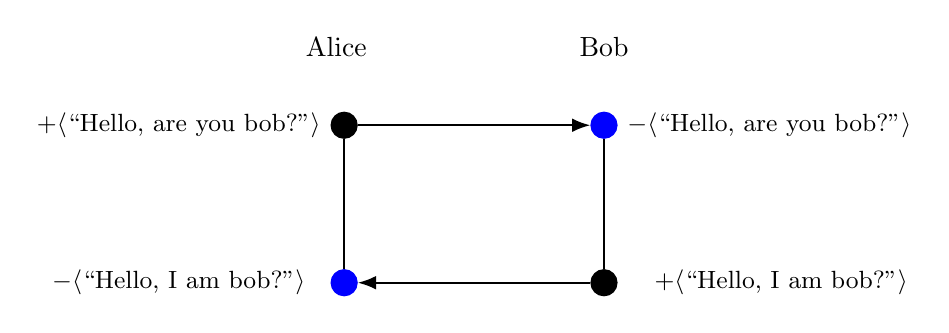
\begin{tikzpicture}
    \node at (2,8) {Alice};
    \node at (0,7) {\small\(+\langle\)``Hello, are you bob?''\(\rangle\)};    \node[shape=circle,draw=blue, fill=blue] (1) at (2.1,5) {};
    \node at (0,5) {\small\(-\langle\)``Hello, I am bob?''\(\rangle\)};
    \node[shape=circle,draw=black, fill=black] (4) at (2.1,7) {};

    \node at (5.4,8) {Bob};
    \node at (7.5,7) {\small \(-\langle\)``Hello, are you bob?''\(\rangle\)};
    \node[shape=circle,draw=black, fill=black] (2) at (5.4,5) {};
    \node at (7.65,5) {\small \(+\langle\)``Hello, I am bob?''\(\rangle\)};
    \node[shape=circle,draw=blue, fill=blue] (3) at (5.4,7) {};

    \path [-,thick](3) edge (2);
    \path [saiarrow](2) edge (1);
    \path [-,thick](1) edge (4);
    \path [saiarrow](4) edge (3);
\end{tikzpicture}
\end{frame}

\begin{frame}\frametitle{Strands can lie}
\hspace{-2.2em}
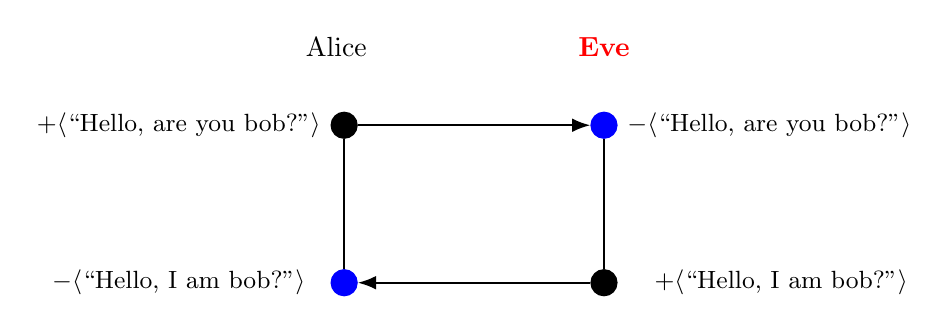
\begin{tikzpicture}
    \node at (2,8) {Alice};
    \node at (0,7) {\small\(+\langle\)``Hello, are you bob?''\(\rangle\)};    \node[shape=circle,draw=blue, fill=blue] (1) at (2.1,5) {};
    \node at (0,5) {\small\(-\langle\)``Hello, I am bob?''\(\rangle\)};
    \node[shape=circle,draw=black, fill=black] (4) at (2.1,7) {};

    \node at (5.4,8) {\isred{Eve}};
    \node at (7.5,7) {\small \(-\langle\)``Hello, are you bob?''\(\rangle\)};
    \node[shape=circle,draw=black, fill=black] (2) at (5.4,5) {};
    \node at (7.65,5) {\small \(+\langle\)``Hello, I am bob?''\(\rangle\)};
    \node[shape=circle,draw=blue, fill=blue] (3) at (5.4,7) {};

    \path [-,thick](3) edge (2);
    \path [saiarrow](2) edge (1);
    \path [-,thick](1) edge (4);
    \path [saiarrow](4) edge (3);
\end{tikzpicture}
\end{frame}

\begin{frame}\frametitle{CPSA adversarial strand actions}

\begin{columns}
\column{0.6\textwidth}
\begin{enumerate}
\item[M.] Text Message: \( \langle +t \rangle \) where \(t \in T\)

\item[T.] Tee: \( \langle -g, +g, +g \rangle \) where \(g \in G\)

\item[C.] Concatenation: \( \langle -g, -h, +gh \rangle \) where \(g,h, gh \in G\)

\item[S.] Separation into components: \( \langle -gh, +g, +h \rangle \)

\item[K.] Key: \( \langle +K \rangle \) where \(K \in \mathbf{K_p}\)

\item[E.] Encryption \( \langle -K, -h, +\{h\}_K \rangle \)

\item[D.] Decryption \( \langle -K^{-1}, -\{h\}_K, +h \rangle \)
\end{enumerate}

\column{0.4\textwidth}

\begin{enumerate}
\item \(\langle +m \rangle\) emit a message from the network.

\item \(\langle -m \rangle\) extract a message from the network.

\item \(\langle +m \rangle\) concatenate two messages.

\item \(\langle +m \rangle\) encrypt a message \(m\) under key \(K\).
\end{enumerate}
\end{columns}
\end{frame}

\begin{frame}\frametitle{An adversarial model of the network}
\pause
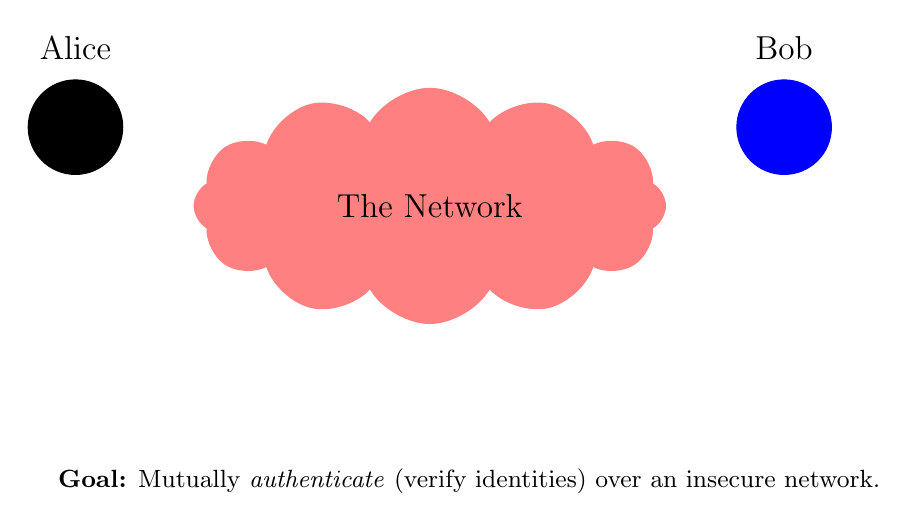
\begin{tikzpicture}[
    node distance=2cm,
    every node/.style={font=\small},
    dot/.style={circle, minimum size=1.2cm, inner sep=0pt},
    arrow/.style={-{Latex[length=4mm]}, very thick}
]

% Left side (Alice)
\node at (0,5.5) {\large Alice};
\node[shape=circle,draw=black,fill=black,minimum size=1.2cm] (1) at (0,4.5) {};
% Right side (Bob)
\node at (9,5.5) {\large Bob};
\node[shape=circle,draw=blue,fill=blue,minimum size=1.2cm] (3) at (9,4.5) {};
% Network cloud
\node[cloud, cloud puffs=12, cloud puff arc=120,
      aspect=2, draw=none, fill=red!50, minimum width=6cm, minimum height=3cm]
      (net) at (4.5,3.5) {\large The Network};

\node at (5,0) {\textbf{Goal:} Mutually \emph{authenticate} (verify identities) over an insecure network.};

\end{tikzpicture}

\end{frame}

\begin{frame}\frametitle{Needham Schroeder}
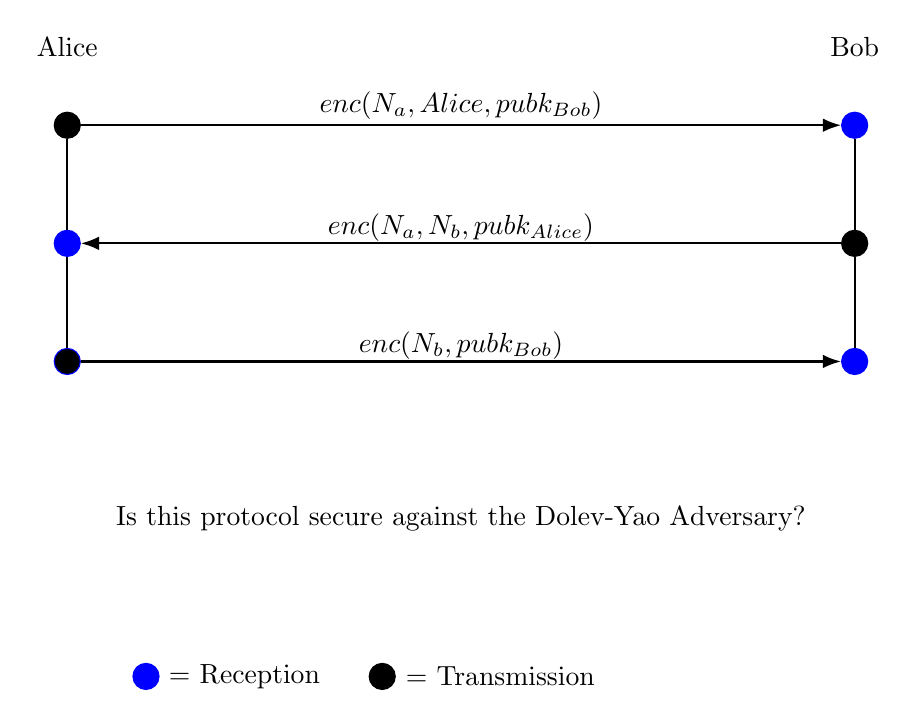
\begin{tikzpicture}
    \node at (0,8) {Alice};
    \node at (10,8) {Bob};
    \node[shape=circle,draw=blue, fill=blue] at (1,0) {};
    \node at (2.25,0) {= Reception};
    \node[shape=circle,draw=black, fill=black] at (4,0) {};
    \node at (5.5,0) {= Transmission};

    \node[shape=circle,draw=black, fill=black] (1) at (0,7) {};
    \node[shape=circle,draw=blue, fill=blue] (2) at (10,7) {};
    \path [saiarrow](1) edge (2);
    
    \node at (5,7.25) {\(enc(N_a, Alice, pubk_{Bob})\)};

    \node[shape=circle,draw=black, fill=black] (3) at (10,5.5) {};
    \node[shape=circle,draw=blue, fill=blue] (4) at (0,5.5) {};
    
    \path [-,thick](3) edge (2);
    \path [saiarrow](3) edge (4);
    \path [-,thick](1) edge (4);
    
    \node at (5,5.7) {\(enc(N_a,N_b,pubk_{Alice})\)};

    \node[shape=circle,draw=blue, fill=black] (5) at (0,4) {};
    \node[shape=circle,draw=blue, fill=blue] (6) at (10,4) {};
    
    \path [-,thick](6) edge (3);
    \path [saiarrow](5) edge (6);
    \path [-,thick](5) edge (4);
    
    \node at (5,4.2) {\(enc(N_b,pubk_{Bob})\)};
    \node at (5,2) {Is this protocol secure against the Dolev-Yao Adversary?};
    
\end{tikzpicture}
\end{frame}

\begin{frame}\frametitle{Needham Schroeder}
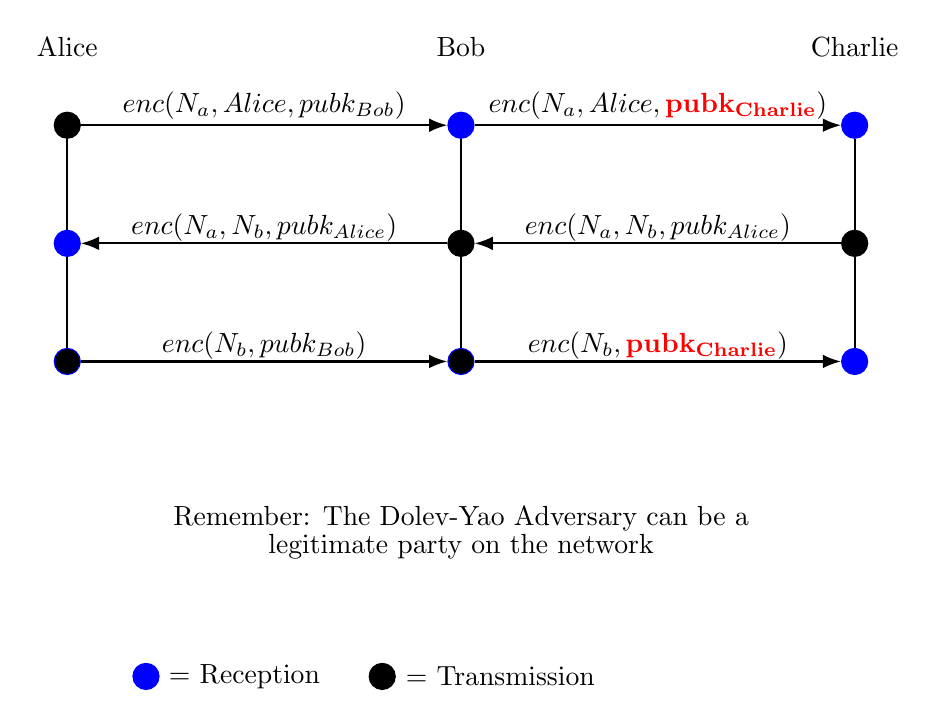
\begin{tikzpicture}
    \node at (0,8) {Alice};
    \node at (10,8) {Charlie};
    \node at (5,8) {Bob};
    \node[shape=circle,draw=blue, fill=blue] at (1,0) {};
    \node at (2.25,0) {= Reception};
    \node[shape=circle,draw=black, fill=black] at (4,0) {};
    \node at (5.5,0) {= Transmission};

    \node[shape=circle,draw=black, fill=black] (1) at (0,7) {};
    \node[shape=circle,draw=blue, fill=blue] (2) at (10,7) {};
    \node[shape=circle,draw=blue, fill=blue] (1m) at (5,7) {};
    
    \path [saiarrow](1) edge (1m);
    \path [saiarrow](1m) edge (2);
    
    \node at (2.5,7.25) {\(enc(N_a, Alice, pubk_{Bob})\)};
    \node at (7.5,7.25) {\(enc(N_a, Alice, \isred{pubk_{Charlie}})\)};
    
    \node[shape=circle,draw=black, fill=black] (3) at (10,5.5) {};
    \node[shape=circle,draw=blue, fill=blue] (4) at (0,5.5) {};
    \node[shape=circle,draw=black, fill=black] (3m) at (5,5.5) {};
    
    \path [-,thick](3) edge (2);
    \path [saiarrow](3) edge (3m);
    \path [saiarrow](3m) edge (4);
    \path [-,thick](1) edge (4);
    \path [-,thick](1m) edge (3m);
    
    \node at (7.5,5.7) {\(enc(N_a,N_b,pubk_{Alice})\)};
    \node at (2.5,5.7) {\(enc(N_a,N_b,pubk_{Alice})\)};

    \node[shape=circle,draw=blue, fill=black] (5) at (0,4) {};
    \node[shape=circle,draw=blue, fill=blue] (6) at (10,4) {};
    \node[shape=circle,draw=blue, fill=black] (5m) at (5,4) {};
    
    \path [-,thick](6) edge (3);
    \path [saiarrow](5) edge (5m);
    \path [saiarrow](5m) edge (6);
    \path [-,thick](5) edge (4);
    \path [-,thick](3m) edge (5m);
    
    \node at (2.5,4.2) {\(enc(N_b,pubk_{Bob})\)};
    \node at (7.5,4.2) {\(enc(N_b,\isred{pubk_{Charlie}})\)};

    \node at (5,2) {Remember: The Dolev-Yao Adversary can be a };
    \node at (5,1.65) {legitimate party on the network};
    
\end{tikzpicture}
\end{frame}

\begin{frame}\frametitle{What do we give CPSA?}
\texttt{protocol.scm}
\begin{itemize}
\pause
\item herald
\pause
\item defmacro
\pause
\item defprotocol
\pause
\item defskeleton
\item defstrand
\end{itemize}
\end{frame}

\begin{frame}\frametitle{What does CPSA give us?}
\texttt{protocol.scm} \(\rightarrow\)

\pause
\begin{itemize}
\item \texttt{protocol.txt}
\pause
\item \texttt{protocol\_shapes.txt}
\pause
\item \texttt{protocol.xhtml}
\pause
\item \texttt{protocol\_shapes.xhtml}
\end{itemize}
\end{frame}

\begin{frame}\frametitle{How can we spot attacks?}
\pause
\begin{itemize}
\item \emph{SECURITY GOALS}
\pause
\item Red circles
\pause
\item Dotted lines
\pause
\item Listener Strands
\end{itemize}
\end{frame}

\begin{frame}\frametitle{Homework}
\pause
\begin{center}
{\Huge Find attacks in CPSA}
\end{center}
\pause
Looking at shapes to find attacks takes some practice, so let us do some practice!

Three of the protocols are already done, you just have to run \texttt{make} so CPSA can make shapes, and then analyze them.

Two of the protocols need to be filled in, you will have to add part of a role, fill in a skeleton, or something else (documented in the comments and README), and then run CPSA to analyze the shapes.
\end{frame}

\begin{frame}\frametitle{Survey}
Fill in details about the survey here!
\end{frame}

\end{document}